\noindent
\begin{tabular}{cc}
\begin{minipage}[b]{0.60\textwidth}
\begin{exerciseS}[Venturi]
Determinare la portata d'acqua che scorre all'interno del tubo di Venturi 
rappresentato in figura, quando sia trascurabile ogni effetto dissipativo 
all'interno della corrente e la velocit\`{a} uniforme nelle sezioni considerate e
a monte del Venturi.
Dati: densit\`{a} dell'acqua $\overline{\rho}= 999\ kg/m^3$, 
densit\`{a} dell'aria $\overline{\rho}= 1.225\ kg/m^3$,
diametro del tubo $D=2\  cm$, diametro della sezione di gola
$d=1\ cm $, altezze: $z_1 = 10\ cm $, $z_2 = 1.2\  m $,
$z_3 = 5\ cm $, $z_4 = 0.5\ m $.

($Q=3.01\, 10^{-4}\ m/s$, $\overline{Q}=3.005\, 10^{-1}\ kg/s$)
\end{exerciseS}
\end{minipage}
&
\begin{minipage}{0.35\textwidth}
   \begin{center}
   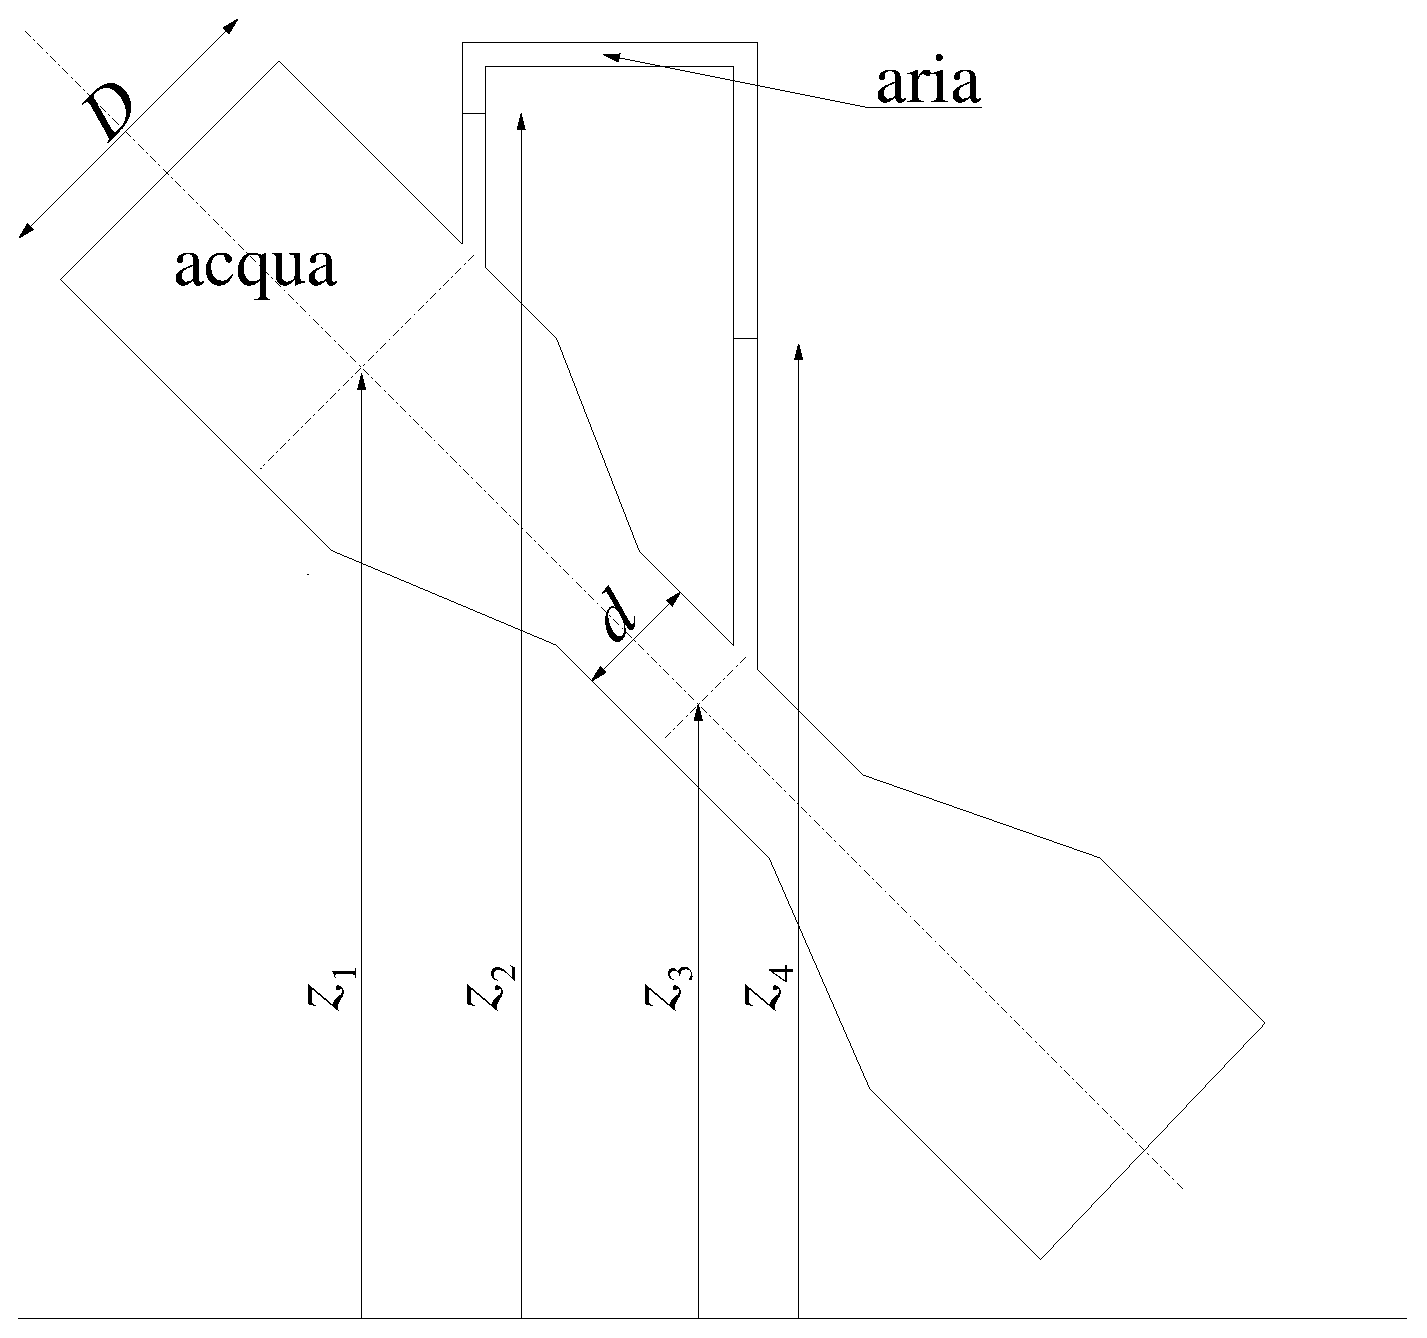
\includegraphics[width=0.90\textwidth]{./fig/venturi.eps}
   \end{center}
\end{minipage}
\end{tabular}

\sol

\partone
Teorema di Bernoulli. Equazione della vorticità. Conseguenze delle ipotesi di stazionarietà, fluido incomprimibile, non viscoso, irrotazionale. Dominio di applicabilità del teorema di Bernoulli. Condizioni all'interfaccia.
Legge di Stevino.

\parttwo
Il problema viene risolto in diversi passi successivi: in principio vengono fatte alcune ipotesi semplificative ($\rho = \bar{\rho}$, $\mu=0$, $\frac{\partial}{\partial t}=0$); poi si utilizza l'equazione della vorticità per semplificare ulteriormente il problema; si determina il dominio in cui è applicabile il teorema di Bernoulli con le ipotesi fatte; si osserva che la parte restante del problema è un problema di statica; si determinano le condizioni di interfaccia tra i due domini; solo a questo punto è possibile scrivere il sistema di equazioni dal quale ricavare le quantità richieste dal problema.

\begin{itemize}

\item 
Il testo del problema consente di fare le seguenti ipotesi: fluido incomprimibile, non viscoso, stazionario. 

\item
L'ipotesi di flusso non viscoso e quella di velocità uniforme a monte permettono di definire il domino all'interno del quale è possibile applicare il teorema di Bernoulli, aggiungendo l'ipotesi di irrotazionalità alle tre ipotesi precedenti. Infatti, l'equazione della vorticità può essere scritta come:
\begin{equation}
  \frac{D \bm{\omega}}{Dt} = (\bm{\omega} \cdot \bm{\nabla}) \bm{u}
\end{equation}
La derivata materiale rappresenta la variazione di una quantità associata a una particella materiale che segue il moto del fluido. Poiché la vorticità nella sezione a monte è nulla (il profilo di velocità è uniforme quindi le derivate spaziali sono nulle), la vorticità rimane nulla ($\frac{d f}{d t} = a f$, se $f=0$ all'istante iniziale la sua derivata in quell'istante è nulla, quindi $f$ non varia, quindi rimane uguale a zero).

\item
Il dominio in cui è possibile applicare il teorema di Bernoulli con le ipotesi di incomprimibilità, assenza di viscosità ed effetti dissipativi, stazionarietà, \textbf{irrotazionalità} e connessione semplice del dominio, coincide con il tubo di Venturi stesso. Infatti in corrispondenza delle prese a parete cade l'ipotesi di irrotazionalità.

Secondo le ipotesi fatte il fluido è non viscoso. Questo assicura che la vorticità sia nulla lungo le linee di corrente. Nel tubo del manometro però il fluido è fermo. Per un fluido non viscoso in corrispondenza dell'interfaccia non ci deve essere discontinuità nella componente normale all'interfaccia stessa e nella pressione. La componente normale è nulla da entrambe le parti della discontinuità; la componente tangenziale è però discontinua: mentre nel tubo di Venturi è diversa da zero, nel tubo del manometro è nulla. Questo comporta che la vorticità non sia nulla (bensì infinita: "differenza finita in uno spessore infinitesimo") e di conseguenza la non validità in questa regione delle ipotesi fatte in precedenza. 

Si possono quindi distinguere due regioni (il tubo di Venturi e il manometro) che non possono "parlare" tra di loro con il teorema di Bernoulli, ma solo tramite la condizione di \textbf{interfaccia} (continuità degli sforzi: per fluidi non viscosi questa condizione coincide con la continuità della pressione).

\begin{figure*}
\centering
\subfloat[][\emph "Suddivisione" del dominio: in tonalità rosse il dominio nel quale è lecito applicare le leggi della statica, in tonalità blu quello nel quale viene applicato il teorema di Bernoulli.]
   {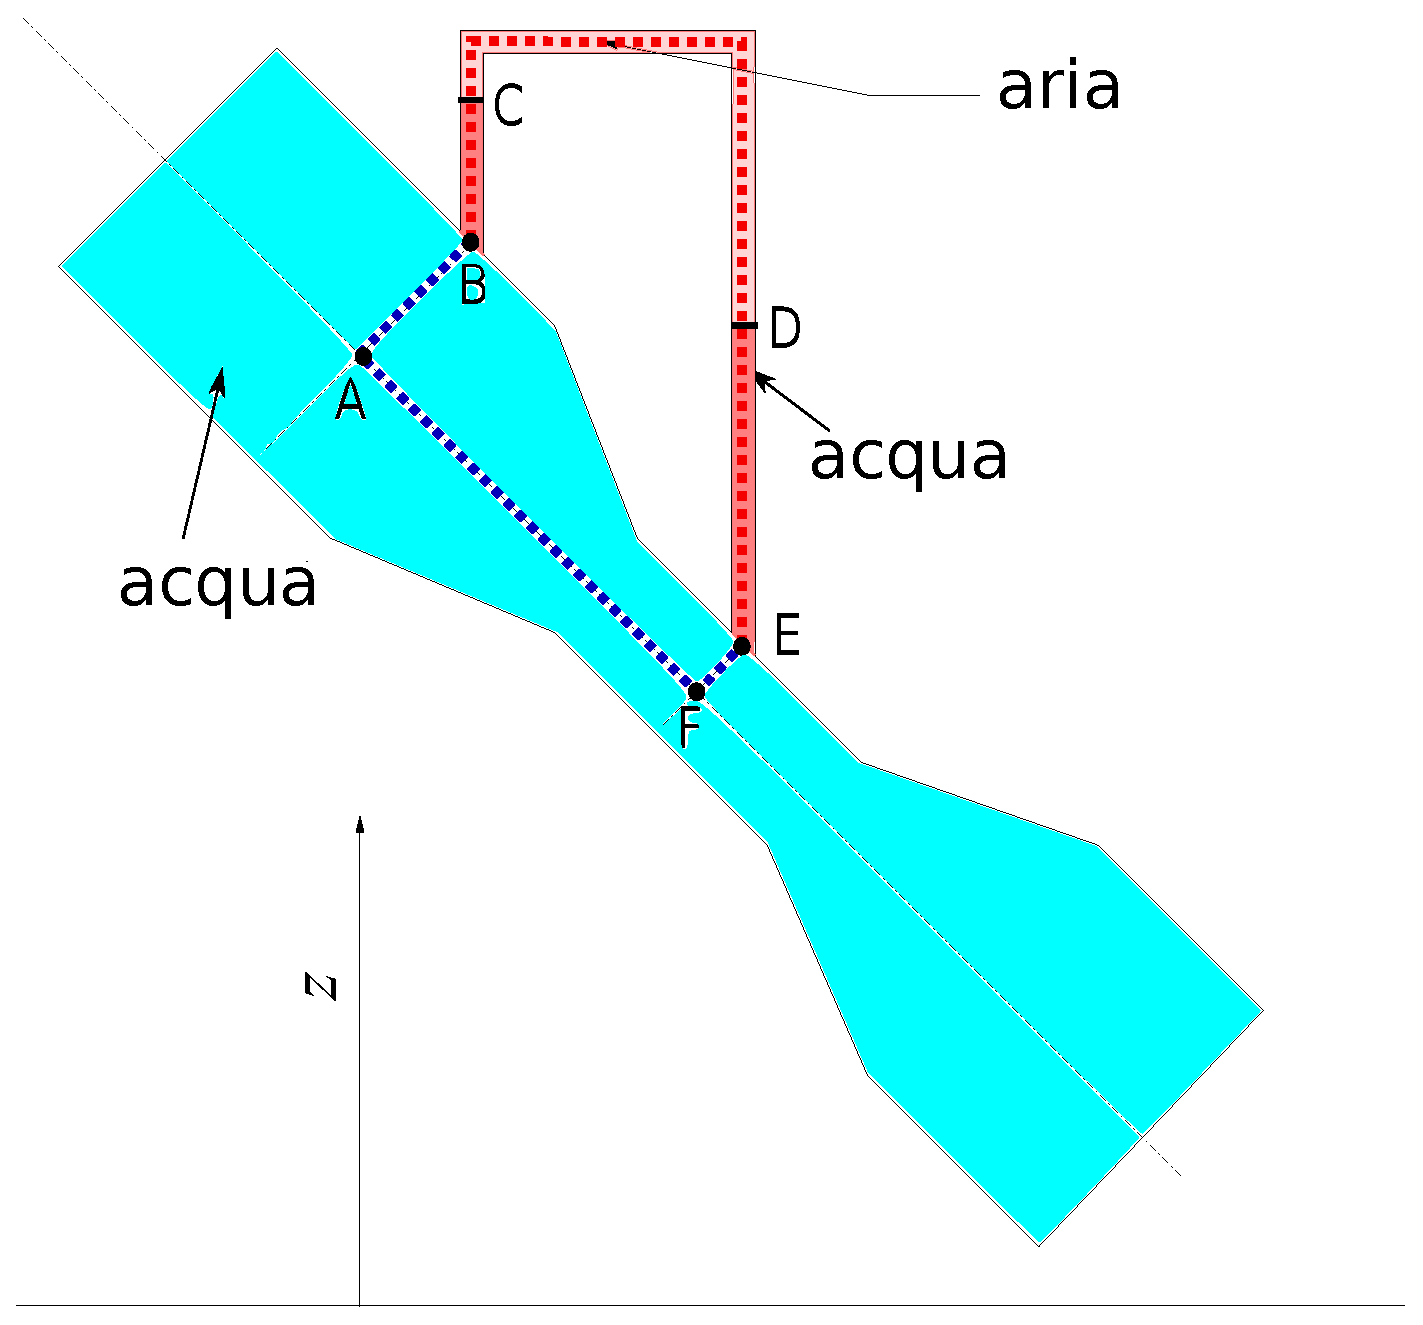
\includegraphics[width=.40\textwidth]{./fig/venturiDomain.eps}} \quad
\subfloat[][\emph Condizioni all'interfaccia. Superficie di discontinuità di velocità e vorticità infinita; la pressione invece è continua. I punti $B_1$ e $B_2$ identificano lo stesso punto al di qua e al di là dell'interfaccia.]
   {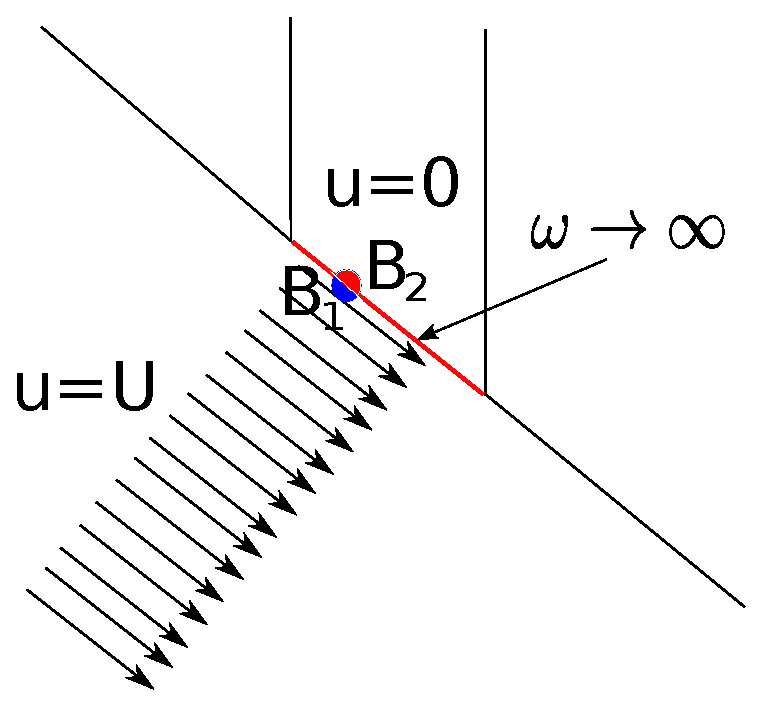
\includegraphics[width=.40\textwidth]{./fig/Discont.eps}}
\end{figure*}

\item \'E possibile ora scrivere il sistema risolvente:

\begin{equation}
\begin{cases}
 P_A + \frac{1}{2}U_A^2 + \rho g z_A = P_{B_1} + \frac{1}{2}U_{B_1}^2 + \rho g z_{B_1} & \text{(Bernoulli A-$B_1$)} \\
 P_{B_1} = P_{B_2} & \text{(interfaccia $B_1$-$B_2$)} \\
 P_{B_2} + \rho g z_{B_2} = P_C + \rho g z_C & \text{(Stevino $B_2$-C)} \\
 P_C + \rho_a g z_C = P_D + \rho_a g z_D & \text{(Stevino C-D)} \\
 P_D + \rho g z_D = P_{E_2} + \rho g z_{E_2} & \text{(Stevino D-$E_2$)} \\
 P_{E_2} = P_{E_1} & \text{(interfaccia $E_2$-$E_1$)} \\
 P_{E_1} + \frac{1}{2} \rho U_{E_1}^2 + \rho g z_{E_1} = P_F + \frac{1}{2} \rho U_F^2 + \rho g z_F & \text{(Bernoulli $E_1$-F)} \\
 P_A + \frac{1}{2}\rho U_A^2 + \rho g z_A = P_F + \frac{1}{2}\rho U_F^2 + \rho g z_F & \text{(Bernoulli A-F)} \\
 \rho \frac{\pi D^2}{4} U_A = \rho \frac{\pi d^2}{4} U_F & \text{(continuità A-F)}
\end{cases}
\end{equation}
che, osservando che $z_{B_1} = z_{B_2} = z_B$, $z_{E_1} = z_{E_2} = z_E$ e applicando le ipotesi fatte in precedenza ($U_A = u_{B_1}$, $U_F = u_{E_1}$, $P_{B_1} = P_{B_2} = P_B$, $P_{E_1} = P_{E_2} = P_E$), diventa:

\begin{equation}
\begin{cases}
 P_A + \rho g z_A = P_{B} + \rho g z_{B} & \text{(Bernoulli A-B)} \\
 P_{B_2} + \rho g z_{B} = P_C + \rho g z_C & \text{(Stevino B-C)} \\
 P_C + \rho_a g z_C = P_D + \rho_a g z_D & \text{(Stevino C-D)} \\
 P_D + \rho g z_D = P_{E} + \rho g z_{E} & \text{(Stevino D-E)} \\
 P_{E_1} + \rho g z_{E} = P_F +  + \rho g z_F & \text{(Bernoulli E-F)} \\
 P_A + \frac{1}{2} \rho U_A^2 + \rho g z_A = P_F + \frac{1}{2}\rho U_F^2 + \rho g z_F & \text{(Bernoulli A-F)} \\
 D^2 U_A = d^2 U_F & \text{(continuità A-F)}
\end{cases}
\end{equation}

Anche se il numero di equazioni è minori del numero di incognite, prova che il sistema è indeterminato, si dimostra che $U_A$ e $U_F$ sono determinate (nelle equazioni intervengono sempre differenze di pressioni, ed è questo il motivo dell'indeterminazione).

\item Soluzione del sistema: il sistema può essere risolto come più si preferisce. Per esempio, partendo da quella che può essere una "lettura dello strumento" $\Delta z = z_C - z_D$ e "chiudendo il ciclo ABCDEF":

\begin{equation}
  \rho_a g \Delta z = P_D - P_C
\end{equation}

\begin{equation}
  \begin{cases}
    P_D = P_E + \rho g (h_E - h_D) = P_F + \rho g (h_F - h_D)\\
    P_C = P_B + \rho g (h_B - h_C) = P_A + \rho g (h_A - h_C)\\
  \end{cases} \\
\end{equation}

\begin{equation}
\begin{aligned}
  \Rightarrow \quad P_D - P_C & = (P_F + \rho g h_F) - (P_A + \rho g h_A) + \rho g \Delta z = 
  & \text{(Bernoulli A-F)}\\
   & = \frac{1}{2}\rho U_A^2 - \frac{1}{2}\rho U_F^2 + \rho g \Delta z = 
  & \text{(continuità)}\\
   & = -\frac{1}{2}\rho U_A^2 \displaystyle\left( \frac{D^4}{d^4} - 1 \right) + \rho g \Delta z \\
\end{aligned}
\end{equation}

E quindi: 

\begin{equation}
  (\rho - \rho_a ) g \Delta z = \frac{1}{2}\rho U_A^2 \displaystyle\left( \frac{D^4}{d^4} - 1 \right)
\end{equation}

\begin{equation}
  U_A = \displaystyle\sqrt{\frac{2 (1 - \rho_a / \rho) g \Delta z}{\frac{D^4}{d^4} - 1}}
\end{equation}

Inserendo i valori numerici, si trova: $U = 0.956 m/s$, $Q = 3.0 \cdot 10^{-4} m^3/s$, $\bar{Q} = 3.0 \cdot 10^{-1} kg/s$.

\end{itemize}


\textit{Osservazioni.} \'E importante saper riconoscere i limiti di applicabilità di formule e teoremi nel rispetto delle ipotesi con le quali essi vengono formulati.

Considerazioni analoghe dovranno essere svolte anche in esercizi simili a questo, riguardanti le soluzioni esatte delle equazioni di Navier-Stokes.
